\chapter{Scenarios}
\label{chap:scenarios}
The tool supports multiple configurations and the behaviour will be different for most of these configurations. Three main scenarios 
will be investigated, order based on the network complexity. Within each scenario, different cases will be investigated.
First, only one user with one drone will be present in the network. The network will thereafter be expanded
for multiple users but with still only one drone available. Eventually, also that last restriction will be dropped meaning 
that multiple users with unlimited number of drones are examined. 
Table \ref{table:defaultconf} shows the default values that are always applicable unless mentioned otherwise.

\begin{table}[!htb]
\centering
\begin{tabular}[t]{ll}
        \toprule
        \multicolumn{2}{l}{\textbf{Broadband cellular network}} \\
        \hline
        \hspace{3mm}  technology        & LTE     \\
        \hspace{3mm}  frequency         & 2.6 GHz \\
        \hline
        \multicolumn{2}{l}{\textbf{Carrier}} \\
        \hline  
        \hspace{3mm}  carrier power        & 13.0 A   \\
        \hspace{3mm}  average carrier speed        & 12.0 m/s \\
        \hspace{3mm}  average carrier power usage      & 17.33 Ah    \\
        \hspace{3mm}  carrier battery voltage       & 22.2 V \\
        \hline
        \multicolumn{2}{l}{\textbf{Femtocell antenna}} \\
        \hline  
        \hspace{3mm}  maximum $P_{tx}$          & 33 dBm   \\
        \hspace{3mm}  antenna  direction        & downwards (az: \ang{0}; el: \ang{90})    \\ 
        \hspace{3mm}  gain                      & 4 dBm   \\ 
        \hspace{3mm}  feeder loss               & 2 dBm   \\ 
        \hspace{3mm}  implementation loss       & 0 dBm   \\
        \hspace{3mm}  radiation pattern         & \acs{EIRP} or microstrip patch antenna\\
        \hspace{3mm}  height                    & 100m  \\
        \hline
        \multicolumn{2}{l}{\textbf{\acs{UE} Antenna}} \\
        \hline 
        \hspace{3mm} height                     & 1.5m from the floor       \\ 
        \hspace{3mm} gain                      & 0 dBm   \\ 
        \hspace{3mm} feeder loss               & 0 dBm   \\ 
        \hspace{3mm} radiation pattern         & \acs{EIRP}  \\
        \hspace{3mm} number present in the network         & 224  \\
        \toprule
\end{tabular}
\caption{Overview of default configuration values.}
\label{table:defaultconf}
\end{table}

%%%%%%%%%%%%%%%%%%%%%%%%%%%%%%%%%%%% scenario 1
\section{A Single User}
\label{sec:scenarios_s1}

This first scenario will investigate how $SAR_{10g}$ and power consumption behave in an isolated environment meaning there is no influence 
from other base stations or other \gls{UE}. The tool will provision one single drone and position it directly above the user.
These results will however depend on the position of the user. If the randomly generated location of the user is indoor, 
the flying height of the drone might be obstructed by the building where the user resides, causing the user to become uncovered. If this is not the case,
the expected altitude of the user is half of the height of the building meaning that the user would be closer to the \gls{UABS} as 
if he would have been outdoors. For more consistent results, the user will be positioned outdoor while systematically 
increasing the flying height. 

Another considered variable will be the transmission power of the antenna.
\gls{LTE} makes use of power control meaning that no more power will be used than strictly necessary. The actual 
transmission power therefore ranges between 0 and the maximum input power. This power is zero when either no user is 
present or the user is so far away that the actual transmitted power would exceed the maximum allowed transmission power.
Increasing the maximum transmission power will not influence the actual power consumption or $SAR_{10g}$ because the \gls{UABS} will not use more
than strictly required. It is therefore more useful to match the actual transmission power against a variable flying height.

This scenario investigates $SAR_{10g}$, power consumption and minimal transmission power for two different types of antennae: a 
 fictional \gls{isotropicradiator} and a realistic antenna.
 The used optimization strategy is not important
for this scenario. This is because the
 decision algorithm decides which user needs to be connected to which drone. Since only one user and one
\gls{UABS} are available, both optimization strategies will behave identical. 

The user gets a fixed position. The exact location doesn't matter as long as it is outside. For this experiment is chosen for the 
`Koningin Maria Hendrikaplein', a square just next to the train station of Ghent.  Doing so will force the \gls{UE} 
to always be at the same height of 1.5 meters. An overview can be found in table \ref{table:confOverviewScenario1}

\begin{table}[!htb]
    \begin{minipage}{.5\linewidth}
      \centering
        \begin{tabular}{|l|c|l|}
        \hline
        \textbf{Parameter}              & \textbf{Value}          \\   \hline 
        x position user               & 3.711198       \\    
        y position user               & 51.036747          \\ 
        shadow margin user             & -3.0398193 \\
        number of users                & 1 \\
        \hline
        \end{tabular}
    \end{minipage}%
    \begin{minipage}{.5\linewidth}
      \centering
            \begin{tabular}{|l|l|}
            \hline
            \textbf{Input variables  }              & \textbf{Output variables}          \\   \hline 
            type of antenna                & $SAR_{10g}$               \\ 
            flying height                  & power consumption             \\ 
                                           &  minimal $P_{tx}$ \\ 
                                           & \\
            \hline
            \end{tabular}
    \end{minipage} 
        \caption{Overview of the configuration.}
        \label{table:confOverviewScenario1}
\end{table}

Note that there is no explicit restriction on the number of drones in table \ref{table:confOverviewScenario1}. The deployment tool initially places 
\gls{UABS}s above each user and it is the optimization strategy that decides which of these potential positions will remain in the end solution.
Since there is only one user, there can also be only one drone.


%%%%%%%%%%%%%%%%%%%%%%%%%%%%%%%%%%%% scenario 2


\section{Increasing Traffic with only one Drone available}

This scenario investigates the same behaviour as the previous one. Still with only one drone but for a higher number of users. 
The scenario can be divided into two cases. The first case has a variable 
flying height with a fixed number of 224 users. This is the number of active users on an average day at 5 p.m. implying rush hour and therefore 
resulting in the highest number of simultaneous users for the day \cite{J2}. The other 
case has a fixed flying height of 100 m as recommended by \cite{J2} but with a variable number of users. To force the tool to only use one drone, a facility capacity is set to one 
indicating that there is only one spot available in the facility where the \gls{UABS}s are stored. The tool will still consider as much potential places 
as there are users in the network. But when the optimization algorithm is done, only one drone will remain.

\begin{table}[!htb]
    \begin{minipage}{.5\linewidth}
      \centering
        \begin{tabular}{|l|c|l|}
        \hline
        \textbf{Parameter}              & \textbf{Value}          \\   \hline 
        facility capacity               & 1        \\    
        &  \\ 
        & \\ 
        & \\ 
        \hline
        \end{tabular}
    \end{minipage}%
    \begin{minipage}{.5\linewidth}
      \centering
            \begin{tabular}{|l|l|}
            \hline
            \textbf{Input variables  }              & \textbf{Output variables}          \\   \hline 
            type of antenna                & $SAR_{10g}$               \\ 
            flying height                     & power consumption             \\ 
            number of users                & user coverage            \\
            optimization strategy         &                               \\ 
            \hline
            \end{tabular}
    \end{minipage} 
        \caption{Overview of the configuration.}
        \label{table:confOverviewScenario2}
\end{table}

For both cases, four configurations are possible because there are two antennae available (\gls{isotropicradiator} and a realistic antenna) which can both operate in a power consumption optimized network or an exposure optimized 
network. The $SAR_{10g}$, power consumption and user coverage will be investigated for all four configurations.


%%%%%%%%%%%%%%%%%%%%%%%%%%%%%%%%%%%% scenario 3


\section{Increasing Traffic with an Undefined Amount of Drones}
\begin{table}[!htb]
      \centering
            \begin{tabular}{|l|l|}
            \hline
            \textbf{Input variables  }              & \textbf{Output variables}          \\   \hline 
            type of antenna                & $SAR_{10g}$               \\ 
            flying height                   & power consumption             \\ 
            number of users                & user coverage            \\ 
            optimization strategy           & \\
            \hline
            \end{tabular}
        \caption{Overview of the configuration.}
        \label{table:confOverviewScenario2}
\end{table}

The third scenario implies no budget limitations. The tool can use as much \gls{UABS}s as desired while trying to maximize coverage. 
A \gls{UABS} will be considered above each user as was also the case in scenario 2. However, the last step where the capacity of the facility
was checked and drones got eliminated is omitted here. It is expected that the optimization strategies will perform best for this scenario since the decision algorithm has been written
 with multiple drones in mind.
The scenario can once again be divided into two cases: one with a fixed flying height of 100 m and a variable number of users and a second one with 
a variable flying height and a fixed number of 224 users.
The influence that these input parameters have on the network will be based on the electromagnetic exposure, power consumption, number of drones required and user coverage.

\section{Overview}
Three different scenarios will be investigated where the second and third one, each consist out of two cases. The first case considers a fixed flying height while 
the second one has a fixed population size. Each case consists out of four configurations. An overview of these configurations is given in table \ref{fig:fourCasesMatrix}.

\begin{figure}[h!]
  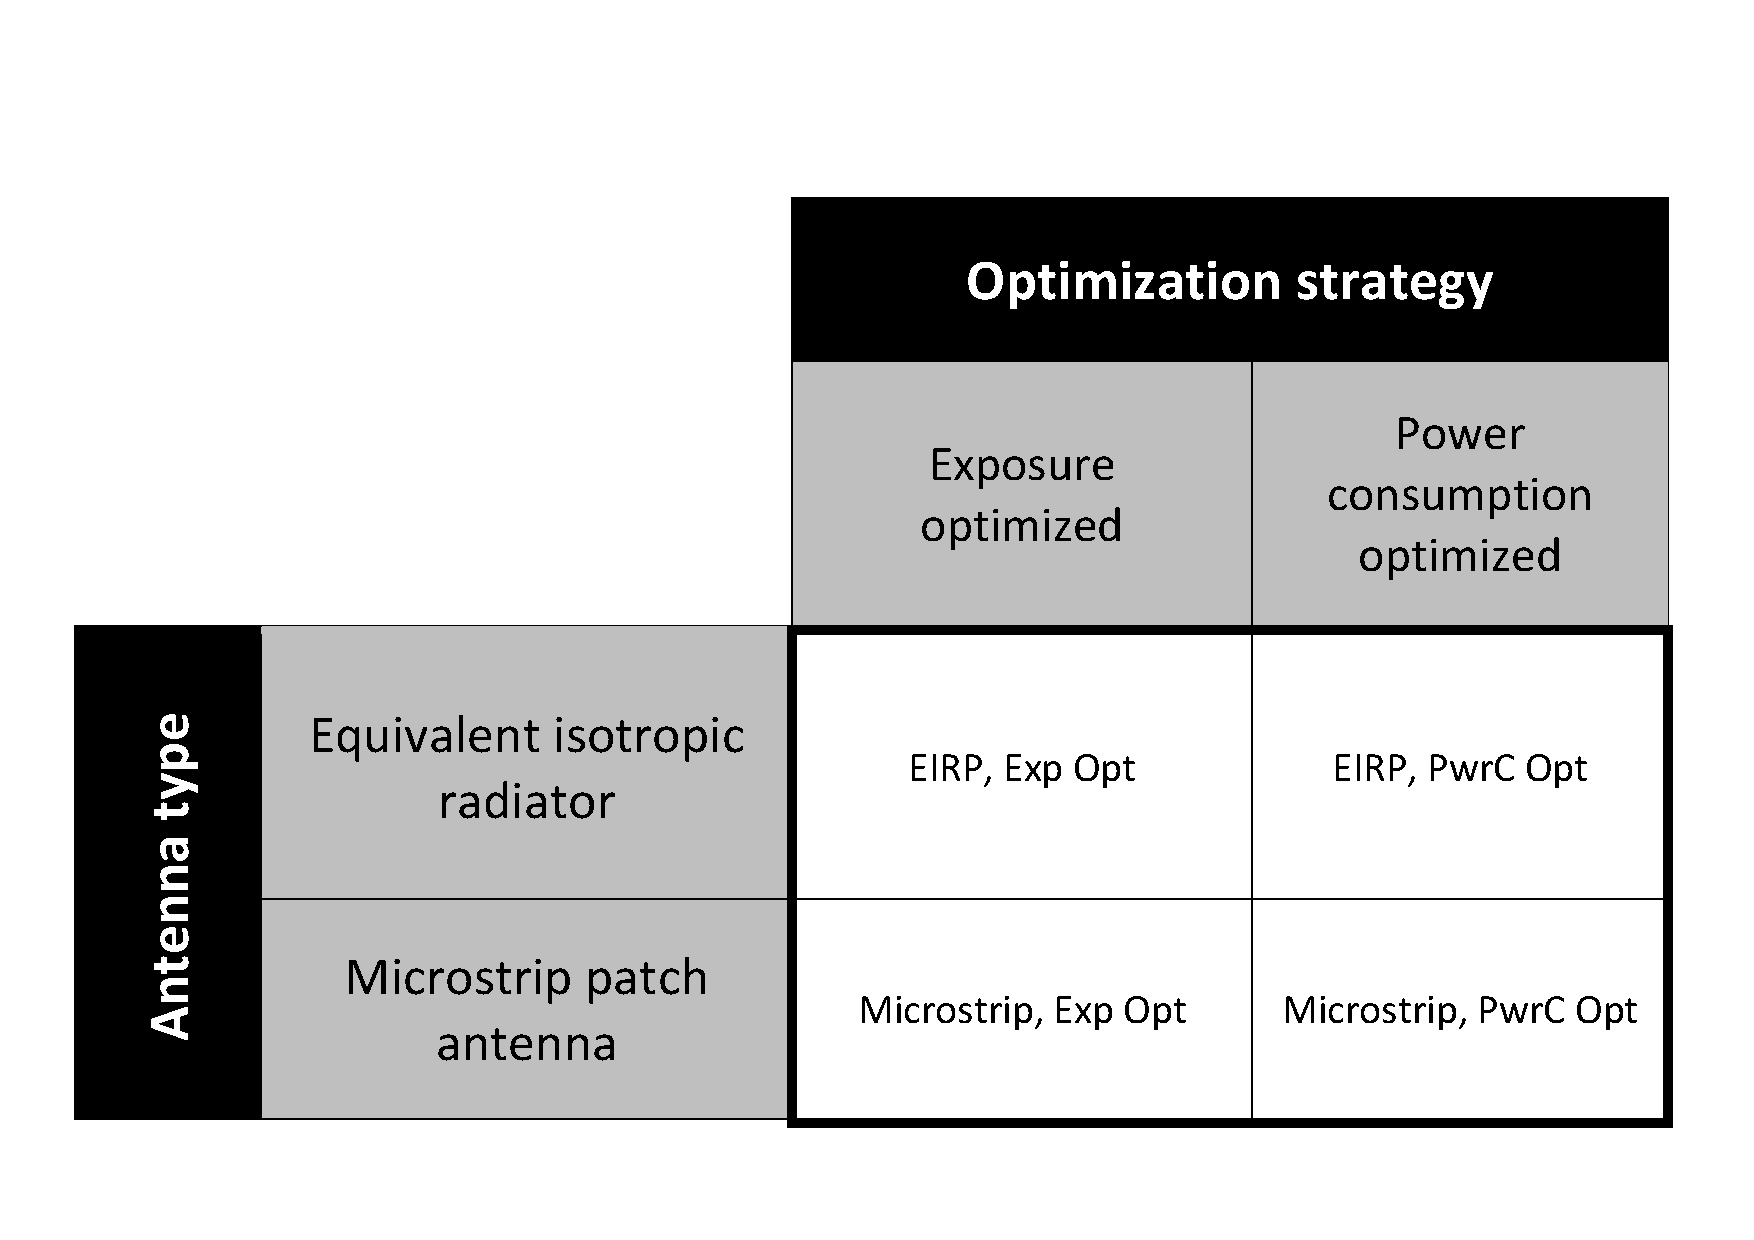
\includegraphics[width=\textwidth]{../images/fourCasesMatrix.pdf}
  \caption{Matrix with the four possible configurations}
  \label{fig:fourCasesMatrix}
\end{figure}